\documentclass[12pt, letterpaper]{article}
\usepackage[utf8]{inputenc}
\usepackage{amsmath}
\usepackage{graphicx}
\graphicspath{ {./slike/} }

\title{Seminarska naloga iz statistike}
\author{Žiga Gladek}

\renewcommand{\refname}{Literatura}

\begin{document}
\maketitle

\renewcommand{\abstractname}{Povzetek}
\begin{abstract}
V tem dokumentu so povzete obravnave nalog, ki sem jih preučeval v sklopu predmeta statistika na programu Matematika UN. Pri reševanju sem si pomagal s programskim jezikom Python, z orodjem Jupyter Notebook in s knjižnico pandas za branje datotek tipa csv. Za prikaze podatkov sem uporabljal knjižnico matplotlib. Za večino uporabljenih metod se sklicujem na zapiske iz predavanj, za preostanek pa na priporočeno literaturo~\cite{Rice}.
\end{abstract}

\section*{1. naloga: Kibergrad}

\subsubsection*{Točka a)} Najprej moramo vzeti enostavni slučajni vzorec $200$ družin in oceniti delež družin v Kibergradu, v katerih vodja gospodinjstva nima mature. Pravi delež bomo označili s $p$. Enostavni slučajni vzorec lahko v programu dobimo s pomočjo ukaza \emph{sample}. Nepristranska ocena za $p$ je:
\[
\hat{p} = \frac{\text{št. gospodinjstev v vzorcu brez mature}}{200}.
\]
Lahko si mislimo, da smo v enostavnem slučajnem vzorcu gospodinjstvom, v katerih ima vodja vsaj maturo, priredili število $0$, tistim, v katerih ima nižjo izobrazbo pa $1$. V tem primeru je ta ocena le povprečje vrednosti v dobljenem vzorcu. Če to implementiramo, nam program pove, da je $\hat{p} = 0,18500$. Seveda pri različnih vzorcih lahko dobimo drugačno oceno, za nadaljnjo obravnavo pa se bomo držali kar te.

\subsubsection*{Točka b)} Ocenili bomo standardno napako, ki je po definiciji enaka $se = \sqrt{var(\hat{p})}$. Naj bo $N$ velikost populacije, $n$ velikost vzorca in $\sigma^2$ populacijska varianca. Potem vemo, da pri enostavnem slučajnem vzorcu velja formula:
\[
se = \sqrt{\frac{N-n}{N-1}\frac{\sigma^2}{n}}.
\]
V resnici pa $\sigma^2$ ne poznamo, zato moramo najprej oceniti še to. V našem primeru, kjer smo vse družine v vzorcu razdelili v dve skupini, velja $\sigma^2 = p(1-p)$. To znamo oceniti s pomočjo $\hat{p}$ kot $\hat{\sigma}^2 = \hat{p}(1 - \hat{p})$, vendar pa ta ocena ni nepristranska. Iz predavanj vemo, da jo lahko do nepristranske popravimo na naslednji način:
\[
\hat{\sigma}^2_+ = \frac{N-1}{N}\frac{n}{n-1} \hat{p}(1 - \hat{p}).
\]
Končno dobimo še nepristransko oceno za standardno napako:
\[
\hat{se}_+ = \sqrt{\frac{N-n}{N}\frac{1}{n-1}\hat{p}(1 - \hat{p})}.
\]
V našem primeru je $N = 43886$ in $n = 200$. Program nam sedaj pove, da je pri danem vzorcu $\hat{se}_+$ enaka približno $0,02746$. Na podlagi te ocene sedaj lahko izpeljemo še $95\%$ interval zaupanja za $p$. Da ga dobimo, bomo upoštevali, da je približno $\frac{\hat{p} - p}{\hat{se}_+} \sim Student(n-1)$. Pri stopnji tveganja $\alpha = 0,05$ dobimo aproksimativni interval zaupanja za $p$:
\[
p \in \left[\hat{p} - F_{Student(199)}^{-1}(0,975)\hat{se}_+, \quad \hat{p} + F_{Student(199)}^{-1}(0,975)\hat{se}_+\right].
\]
Ta je pri danih podatkih enak približno $[0,13062, 0,23938]$. Pri tem smo na podlagi tabele kvantilov Studentove porazdelitve upoštevali, da je $F_{Student(199)}^{-1}(0,975)$ približno enak $1,98$. Dejansko smo uporabili kvantil, ki ustreza $120$ prostostnim stopnjam, vendar je to za naše namene dovolj dober približek.

\subsubsection*{Točka c)} Poglejmo populacijski delež gospodinjstev, v katerih vodja gospodinjstva nima srednješolske izobrazbe. Ta delež je enak:
\[
p = \frac{\text{št. gospodinjstev brez mature}}{N} = 0,21150.
\]
Naša točkovna ocena se od točne vrednosti torej razlikuje za slabe $3\%$, opazimo pa tudi, da prej dobljeni aproksimativni interval zaupanja pokrije populacijski delež.
S tem da poznamo $p$ lahko izračunamo tudi pravo standardno napako pri vzorcih velikosti $200$.
Upoštevajmo, da je $\sigma^2 = p(1-p)$. Tedaj je:
\[
se = \sqrt{\frac{N-n}{N-1}\frac{\sigma^2}{n}} = \sqrt{\frac{N-n}{N-1}\frac{p(1-p)}{n}} \doteq 0,02881.
\]
Približek $\hat{se}_+$ se torej od točne vrednosti razlikuje šele na tretji decimalki.

\subsubsection*{Točka d)} Vzeli bomo še $99$ enostavnih slučajnih vzorcev in za vsakega od teh določili $95\%$ interval zaupanja za $p$. S pomočjo programa dobimo, da je delež intervalov, ki pokrije populacijski delež enak $\frac{95}{100}$. Poglejmo si to še s sliko:
\begin{center}
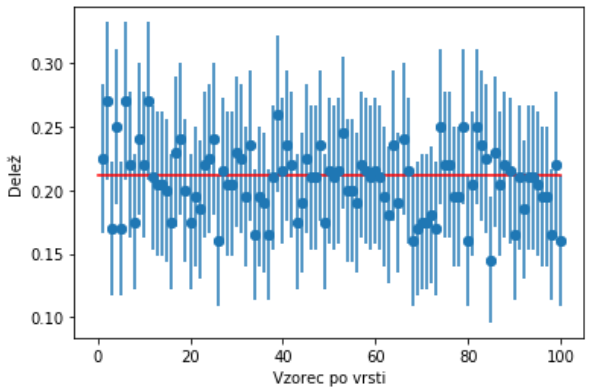
\includegraphics[scale=0.7]{Intervali}
\end{center}
Rdeča črta na sliki prikazuje populacijski delež, intervali zaupanja pa so narisani vertikalno, pri čemer je vrednost na sredini intervala dodatno označena z modro piko. Število intervalov, ki je pokrilo populacijski delež ni presenetljivo in kvečjemu potrdi, da smo pravilno določilli interval zaupanja, saj $95\%$ interval zaupanja pomeni ravno to, da bo populacijski delež pokril v približno $\frac{95}{100}$ primerih.

\subsubsection*{Točka e)} Določimo še standardne odklone za teh $100$ dobljenih vzorcev.



\begin{thebibliography}{99}
\bibitem{Rice} J. A.~Rice, \emph{Mathematical Statistics and Data Analysis, Third Edition}, Thomson Brooks/Cole, Duxbury, 2007
\end{thebibliography}

\end{document}

